\chapter{On quantitative imaging of single cells}
\label{imaging:introduction}

\section{Introduction}

Fluorescence microscopy is a
powerful tool for measuring single-cell properties, especially when sub-cellular
spatial resolution is required. With modern computing
power and robotics, we can now use this technology to amass large
quantities of image data and so study
cell biology with increasing breadth and depth. 
Accurate high-throughput imaging and image analysis of single-cell data across
large numbers of conditions is becoming routine in
some labs and will continue to become even more commonplace
as the technology simultaneously improves and becomes cheaper.
The availability of the technology has led, in recent years, to a boom
in large-scale microscopy studies of single-cell phenotypes
\cite{Neumann2006,Young2008,Feng2009,Houle2010,Held2010,Singh2010,Futamura2012}.
However, our ability to generate
microscopy data is outpacing our collective ability to
analyze and interpret it.


Fluorescence microscopy has been an experimental staple of biology for many years,
though it is still infrequently used for rigorous quantitative analysis. More often,
researchers use fluorescence imaging to demonstrate a particular phenotype
(as I do in \ar{fig:insulation:schematic}),
or to manually count the instances of a visually obvious
phenotype. Our own visual perception is notoriously prone to error, however,
as our brains can choose to perceive patterns that do not exist, thus
allowing for latent biases to affect how we manually tally the data.
As biologists we are often painfully aware of this problem,
and so there seems to be a general unease when it comes
to evaluating imaging data. We all know the joke that,
in published figures, ``representative image'' is a euphemism for
``the best image I could find.''


The distrust is understandable, as proper evaluation
of imaging data is a non-trivial task, and researchers
rarely publish enough details to even allow
for thorough evaluation in the first place. This problem is 
made worse by a lack of imaging and analysis standards, and by the
difficulty inherent to making large image-datasets publicly available.


Biological image
quantification is a difficult and generally unsolved problem \cite{Danuser2011},
and its various approximate
solutions tend to require a level of expertise in mathematics
and computer programming, and at least a cursory
understanding of microscopy optics. Importantly, it also requires expertise
in the experimental biology under study. Few, if any, biology training
programs prepare students for such broad practical knowledge.


Cell biologists, like myself,
are rarely trained in quantitative fields
and so we tend to rely on our colleagues
in analytical fields to do the quantitative work for us. Those analysts,
in turn, typically lean back on the biologists for understanding the
``what'' and ``why'' of the analysis.
Unfortunately, the large knowledge and language
asymmetry between biologists and analysts
creates steep communication barriers that are hard to break
down. Therefore, the full benefits to cell biology of careful
quantitative microscopy may be going untapped.


My own work relies almost entirely on imaging (\ar{insulation:introduction})
and, having spent so much time thiking about and performing image analysis,
I have come to prefer imaging over other methods not only for its efficiency
in measuring single-cell properties across large numbers
of conditions, but also because it provides a literal view into
the mysterious and beautiful world of the cell. I therefore hope that
careful single-cell image analysis will someday become as commonplace as Western
blots.


My overarching goal in writing this chapter is to provide
an image analysis resource that is both accessible
to classically trained biologists
and useful for analysts from non-biological fields
that may be preparing to move into the field. In general, I aim to provide careful
biological and analytical
reasoning for a subset of the many choices that must
be made with respect to
fluorescence imaging experiments. In specific, I focus
on dealing with
experimental and imaging artifacts and noise,
and how to choose biologically meaningful single-cell
measurements. The methods and rationale in this chapter
are used extensively in \ar{insulation:introduction}.



\section{Images as layers of fluorescence}
\label{imaging:model}


The goal of quantitative biological imaging, in overly general terms, is to perform
a set of meaningful mathematical operations on fluorescent images.
We therefore require a mathematical model of fluorescence images
to use as a reference when discussing image correction and analysis.
Note that the model I construct below is designed
to be intuitive with respect to cell culture microscopy,
and so it differs slightly from the
more general models that it is founded upon
\cite{Schultz1974,Madiset1998,L2000,Model2001}.


A fluorescence microscopy image $I$ can be thought of as
a series of fluorescing layers, each with its own distinct properties,
that add together to create the final image \arp{fig:imaging:layers}.
In this simple model, a fluorescence image is composed of multiple
\b{foreground} and \b{background} layers that come 
from distinct components of the sample.
(As described below, I use specific
definitions of these terms ``foreground'' and ``background''
that may differ from one's intuition.)
It is important to note that additivity is a special property
of fluorescence microscopy, as bright-field and other non-fluorescence signals do
not necessarily behave in this way \cite{L2000}.
Further, there are cases where the layers
of fluorescence will become non-additive,
as the fluorophores and the camera
will display non-linear behaviors in certain ranges \cite{Hiraoka1987}. 
The model I describe
here, and all analysis in this chapter, assumes that
all contributing components are behaving within their linear ranges.


  \begin{figure}[!bt]
  \centering
  \includegraphics[width=3in]{FIGS/imaging/layers.pdf}
  {\singlespacing 
  \caption[ Images as layers of fluorscence.]
            { A fluorescence image $I$ of a cell is the sum of
			distinct fluorescence layers. Here,
			$F_1$ is the foreground signal of interest, $F_2$
			is non-specific staining within the cell, and $B$
			is background fluorescence from the imaging surface.}
  \label{fig:imaging:layers}}
  \end{figure}

  
\subsubsection{Experimental image layers $F$ and $B$}


In this dissertation, foreground ($F$) refers
to any image layer that emits fluorescence in a spatially non-uniform manner
within an image; the layer is not ``flat.''
The most useful foreground layer is due to the specific binding of a
fluorescent probe to its target, as this layer is
likely the one that is under study.
Where my definition of ``foreground'' may diverge from others
is that I include spatially non-uniform fluorescence artifacts
as foreground layers. Such artifacts might include
non-specific cellular staining, cellular autofluorescence
(as for layer $F_2$ in \ar{fig:imaging:layers}), and staining artifacts
such as halos, bubbles, or bright puncta.
Many biologists refer to these artifacts
as ``background'', but I have a specific definition for this term as well.


Also specific to this dissertation, ``background'' ($B$) refers to any image
layer that emits fluorescence in a spatially uniform manner within an image
(e.g. layer $B$ in \ar{fig:imaging:layers}).
In other words, the layer is ``flat,'' aside from variation between
pixels due to measurement error.
Background layers may include reflections from the imaging
surface, autofluorescence from unbound fluorophore in the solvent, or fluorophore
that has adhered to the imaging surface.


Finally, all fluorescent image layers scale linearly
with excitation light intensity and
exposure time (again, so long as we are in the
linear range for all image components).
For convenience
we can fold excitation intensity and exposure time into a single term $t$, 
which I refer to simply as ``exposure.'' 
Taken together we get the (yet-incomplete)
image model in \ar{eq:imaging:simpleModel} that contains $n$ foreground
and $m$ background layers.
%
\begin{equation} \label{eq:imaging:simpleModel}
I = t \left( \sum_{i=1}^n F_i + \sum_{j=1}^m B_j \right)
\end{equation}


\subsubsection{Image modification by the microsope}

The model in \ar{eq:imaging:simpleModel} describes the fluorescing
layers of an image, but there are also non-fluorescent properties
of images.
In digital fluorescence microscopy, the camera typically has some
non-zero baseline value that I refer to as the ``detector value'' $D$.
This value is a constant and does not change with
exposure \cite{Goldman2005}.


  \begin{figure}[!bt]
  \centering
  \includegraphics[width=5in]{FIGS/imaging/components.pdf}
  {\singlespacing 
  \caption[ Components of a fluorescence image.]
            { A fluorescence image can be modeled by
            $I=D+S(F+B)$, where $D$ is the baseline detector value,
            $S$ is shading, $F$ is the foreground, and $B$ is the
            background. Here, synthetic images of two foreground
            objects demonstrate each of these
            components. Plots indicate pixel values along the white line
            drawn across the image as i \b{a}. \b{a}, Two foreground objects that
            vary 2-fold in intensity are shown. \b{b}, Addition of
            background reduces the apparent fold-difference between the
            two foreground objects, as does addition of the detector
            (\b{c}). \b{d} Shading distorts the foreground and background,
            but leaves the detector contribution unchanged.}
  \label{fig:imaging:components}}
  \end{figure}



Uneven illumination of the image by the light source,
which I refer to as ``shading'' ($S$),
is an optical problem inherent to microscopy
\cite{Hiraoka1987,Inoue1997,Murray2007,Fiolka2008}. Shading
is a consequence of how light moves through lenses and so it is
not just a property of wide-field microscopy,
though this is a common misconception: shading is also present in confocal
and total internal fluorescence (TIRF) microscopy \cite{Fiolka2008,Herbert2012}.


Shading can be interpreted as variation in relative
exposure as a function of position within the image.
In other words, $S$ modifies
$t$ in a pixel-coordinate dependent manner. Because fluorescence units
are typically arbitrary, in that their absolute values carry
no meaning, I simplify the model further by setting $t=1$
and dropping it from the equation
(note that analyses making use of varied exposure
times could also collapse $S$ and $t$ into a single term).
By including the $S$ and $D$ components,
and a noise term $\epsilon$ to absorb
experimental error, we get the complete model in
\ar{eq:imaging:fullModel}.


I simplify the model further by collapsing all
foreground and background layers into
single terms. The resulting image model in \ar{eq:imaging:simpleFullModel}
is used throughout this text.
This simplification is useful because the basic image
correction and analysis methods presented in this chapter do not
distinguish between foreground layers or between background layers.
It is useful to keep the multi-layer model in mind, however, as
it will help when trying to untangle the overall fluorescence behavior
of experimental images.
See \ar{fig:imaging:components} for a visual
demonstration of the simple model. 


\begin{gather}
I = D + S \left( \sum_{i=1}^n F_i + \sum_{j=1}^m B_j \right)\epsilon  \label{eq:imaging:fullModel} \\
I = D + S (F+B)\epsilon  \label{eq:imaging:simpleFullModel}
\end{gather}


\subsection{Properties of the image components}


With a model in place, it is useful to obtain some intuition for how to
think about images in this framework. First, note that the image itself,
and each layer that makes it up, is a matrix of intensity values
(\ar{fig:imaging:stack}). Many
analytical operations can be performed per pixel coordinate, in effect
ignoring the presence of neighboring pixels.
Other operations take into account
those neighbors (this is especially true of segmentation,
discussed later). Finally, we can think of a ``stack'' of images,
in the same way
one would stack a deck of cards. We can perform operations ``down the
stack'' at particular pixel coordinate.
Such operations include ``per-pixel'' means and medians.


  \begin{figure}[!bt]
  \centering
  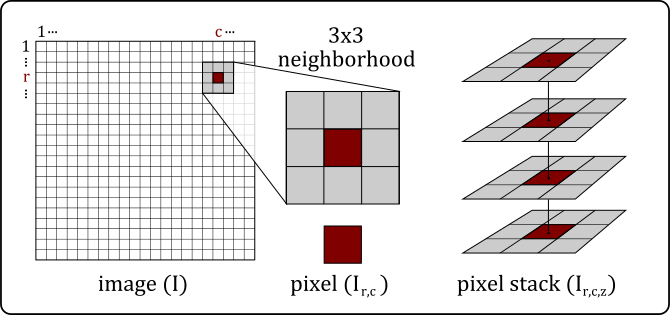
\includegraphics[width=4in]{FIGS/imaging/stack.pdf}
  {\singlespacing 
  \caption[ Pixel coordinate system.]
            { An image $I_{r,c}$ is a matrix of intensity values,
            with pixel coordinates
			given by row $r$ and column $c$. Analyses can
			be performed on single pixels, the entire image, image
			neighborhoods, or image stacks as shown. In the case of an image stack,
			$z$ refers to the image position within the stack. Note that $z$ need not
			refer to a height, as in the common z-stacks of confocal microscopy,
			but can also indicate different color
			channels or even entirely unrelated images. In effect, $z$
            is a ``height'' within the image stack that may not
            correspond to the physical height of an imaged within a sample.}
  \label{fig:imaging:stack}}
  \end{figure}


Each component of the image model in \ar{eq:imaging:simpleFullModel}
is a matrix of the same dimensions,
and each has distinct properties. The foreground components
of $F$ have completely idiosyncratic
values, both within and between images, as these
values depend on where cells are, what is
being stained, and what kinds of randomly-positioned
artifacts are present. Indeed, the
unknown behaviors of the foreground layers are 
what we typically aim to understand
via image analysis.


The background layers of $B$ are defined to
be more predictable, in that they are
unchanging by position within an image. The background should
be constant between images as well,
when identical experimental conditions
are used to obtain those images.
However, the total background
may change as a consequence of some experimental
perturbation. For example, some small
molecules used as drugs may fluoresce
and so add an additional background layer.
Finally, note that due to shading these
``flat'' background layers will appear
distorted in uncorrected images.
To clarify, then, I define background
layers as those that are constant across an image
in the absence of shading.


The detector layer $D$ has the simplest behavior, as it can be considered
constant regardless of the imaging and experimental conditions. ``Constant'' in this
case means that the value at any given pixel position $D_{r,c}$ does not change
over time or between images.
The values within an image, on the other hand, may vary
(see \ar{fig:imaging:properties}a).


The shading value $S$ is problematic for analysis in that it distorts the
$B$ and $F$ layers in non-trivial ways.
Like $D$, this layer also shows variation within an image.
The shading pattern caused by the objective lens
tends to show brighter fluorescence at image centers
and weaker fluorescence at the edges. However,
the presence of other components
in the light path, such as filters, can modify this shading pattern
(\ar{fig:imaging:properties}b) \cite{VandenDoel1998}.
Unlike $D$, the shading pattern can vary between
images as well, though in \ar{imaging:correction} I show that this variation
can be both predictable and correctable. $S$ distorts the $F$ and $B$ layers
multiplicatively, and can cause as
large as 1.5- to 2-fold intensity differences across an image
\cite{Bray2013}.




  \begin{figure}[!bt]
  \centering
  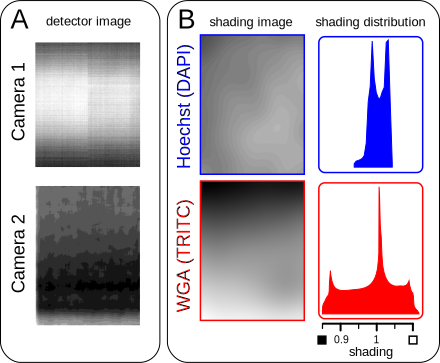
\includegraphics[width=4in]{FIGS/imaging/properties.pdf}
  {\singlespacing 
  \caption[ Example detector $D$ and shading $S$ patterns.]
            { Example within-image variation of the detector $D$
			and shading $S$ image components. \b{a}, Per-pixel
            averages of 10 detector images from
			two cameras are shown. Camera 1, Andor Zyla sCMOS 11-bit.
			Camera 2, Roper Scientific CoolSnap HQ2 CCD 14-bit.
            Intensities and
			images are scaled independently.
			\b{b}, Shading patterns from two optical channels. Uniformly-fluorescent
			background images were made with dissolved Hoechst or wheat
			germ agglutinin (WGA)-TRITC in the DAPI and TRITC optical channels. Note
			that each channel has a dramatically different shading pattern and overall
			degree of shading. Histograms show the all-pixel distributions
			of shading values, which are defined to have
			a median of one (a robust variant of $\E[S]\equiv 1$, defined in
			\ar{imaging:correction}).
			}
  \label{fig:imaging:properties}}
  \end{figure}


Finally, we are left with the noise term $\epsilon$. I use this
term specifically to capture measurement noise, not true biological
variability. The largest source of measurement
noise for modern fluorescence imaging
is probably due to the combination of two factors: the error in converting
photon counts to electrons, and the error introduced during transmission
of those electrons from the camera. Combined, this measurement error
introduces an intensity-dependent uncertainty in the total measured
intensity of the pixel $I_{r,c}$. In general, the relative error
decreases as a function of the square root of intensity \cite{Goldman2005}.




\section{On image correction}
\label{imaging:correction}

Fluorescence microscopy images contain non-biological data,
distortions, and artifacts that may confound analytical results if
not addressed.
In the terms of the image model from the previous section
(\ref{eq:imaging:simpleFullModel}), the
subject of study in fluorescence imaging is contained within a subset of the
foreground layers. All non-foreground components should thus
be removed in order to obtain meaningful quantitative results.
Ideally, the foreground layers that are not of interest (especially
artifacts) should also be removed, though this is a much more difficult
problem that I do not address in this dissertation.
In essence, from the original image $I=D+S(F+B)\epsilon$, we need to
obtain $F$: obtaining $F$ is the goal of image correction.


It is important to be aware that image correction is not a solved
problem. There are many ways in which it can be done, several of which I review
in \ar{imaging:correction:review}, but the most commonly-used methods produce
incomplete correction and/or are prone
to generating artifacts. Further, methods sections of papers that
rely on imaging often do not explain their correction methodology
at all, making it difficult to evaluate some published results.
I therefore make the importance of image correction a focus
of this chapter, and describe an image correction
approach that I developed for accurate determination of $F$
in the difficult context of high-throughput microscopy
\ar{imaging:correction:myMethod} \cite{Coster2014}.


Before going into the details of image correction, I should
first address whether this step is even necessary.
After all, any processing step
could introduce artifacts and thus potentially do more harm than good.
Normal cell-to-cell variability is already relatively high,
with standard deviations of 
$\sim$15-30\% for protein concentrations \cite{Sigal2006a}. One might then
wonder whether error introduced by non-foreground image components
would make much of a difference. Here I show that it can
indeed make a difference. Unsurprisingly,
the size of the difference (and thus the importance) is highly
dependent on the properties of each particular image dataset,
the measurement methods used, and the experimental goals.


\subsection{Non-foreground components distort single-cell phenotypes}
\label{imaging:distortion}


A particular cellular phenotype can be represented
as a set of measurements.
For example, a cell phenotype might be composed of
its measured size, shape, texture,
and average fluorescence intensities in multiple
color channels. Each measurement is
generally referred to as a ``feature.'' The diversity
of features that can be measured
for a  single cell is only limited by the imagination
of the investigator. It would therefore
be impossible to develop a single
comprehensive argument for the importance
of image correction that covers all possible
ways of measuring cellular phenotypes.
Instead, I make a case study of several
commonly-used and biologically-interpretable
single-cell features: the average, total,
and ratios of fluorescence intensity.


    \begin{table}[!bt]
    \caption[Table of symbols for average, total, and ratiometric features.]
    {Symbols used in the mathematical derivations of the consequences of $S$
    and $B$ on single-cell feature distributions.}
    \label{table:imaging:symbols}
    \centering
    \begin{tabular}{cl}
    \hline
    Symbol & Meaning \\ \hline
    $\E[X]$   & Expected value (i.e. the mean) of the random variable $X$ \\
    $F_c$	 & Average foreground intensity within cell $c$ \\
    $S_c$	 & Average shading value within cell $c$ \\
    $B$	     & Background intensity per pixel, a constant\\
    $\alpha_c$ & Area of cell $c$ \\
    $A$	     & Average intensity feature \\
    $T$	     & Total intensity feature \\
    $R$	     & Ratio of intensities feature \\
    $Z_c$    & The value of feature $Z$ for a single cell, $c$.\\
    $\sigma_Z$ & The standard deviation of feature $Z$ across all cells. \\
    $\mu_Z$    & The mean of feature $Z$ across all cells. \\
    $cv_Z$     & The coefficient of variation of feature $Z$ across all cells  ($\sigma_Z/\mu_Z$). \\
    \hline
    \end{tabular}
    \end{table}


How to quantify the effects of image correction on data is not obvious,
since that data can be used in many ways depending on experimental goals.
There are, however, aspects of
single-cell distributions that are meaningful across a broad array of
experiments, and so I use these as metrics when measuring the consequences
of image correction. These are the mean ($\mu$), standard deviation ($\sigma$),
and coefficient of variation ($cv=\sigma/\mu$) of a feature across a population of cells.


The standard deviation and $cv$ are measures of distribution widths, which
are used to determine the statistical separability of distributions.
Inaccurate measurements of the true variability may
consequently reduce statistical power.
The mean of a feature distribution, on the other hand,
is typically used to determine how large of an
effect an experimental perturbation has had. Inaccurate measurements of the true mean
may cause strong results to appear weak, or vice versa, leading to false
negatives or false positives. These distribution metrics are
therefore useful as readouts for the utility of image correction.


The mathematics in the following discussion were
worked out in conjunction with my co-authors on the relevant
publication \cite{Coster2014}: Satwik Rajaram, Chonlarat Wichaidit,
Steven Altschuler, and Lani Wu. The text
and figures draw heavily from the same publication. Those readers
who do not need convincing that image correction is important may skip
to page~\pageref{imaging:correction:review} without a loss in coherence
of this chapter.


  \begin{figure}[!bt]
  \centering
  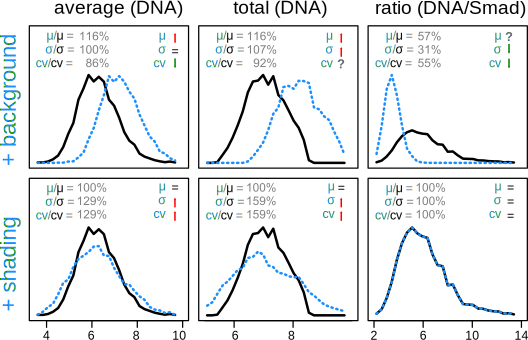
\includegraphics[width=4.5in]{FIGS/imaging/SBeffects.pdf}
  {\singlespacing 
  \caption[ Case study of the effects of $S$ and $B$ on single-cell features.]
            { Image background and shading cause feature-dependent changes
            in estimates of phenotypic variability.
            Human colonic epithelial cells ($n>3700$), stained for DNA
            (using Hoechst) and Smad (using a Smad2/3 antibody), imaged
            at 10X.
            The distributions of
            nuclear feature values were then compared
            before (black histograms) and after (dotted blue histograms)
            artificial background (top row, with
            background $\sim$16\% of Hoechst or $\sim$50\% of Smad foreground)
            or shading (bottom row, linear
            gradient with maximum 1.5 fold intensity difference) were added
            to each image. $\mu$, mean; $\sigma$, standard deviation;
            $cv=\sigma/\mu$. Inset, top left,
            relative size of change to the shown distributions. Inset, top right,
            arrows indicate the direction of
            change in the general case (question marks indicate uncertainty due to
            dependency on other variables). $x$-axes in arbitrary fluorescence units.
            A version of this figure is published as Fig. 1a in \cite{Coster2014}.}
  \label{fig:imaging:SBeffects}}
  \end{figure}





\subsubsection{Mathematical definitions of commonly used single-cell features}


Commonly used single-cell measurements include pixel intensity averages,
totals, and ratios within some cellular compartment $c$ (such as the
nucleus, cytosol, or whole cell).
By defining these features mathematically we
can determine their general behaviors as a consequence of the presence of image background
or shading. Refer to \ar{table:imaging:symbols} for the list of mathematical
symbols, to \ar{table:imaging:properties} for a summary of the statistical
properties used in the mathematical derivations, and
\ar{fig:imaging:SBeffects} for a case study of these behaviors.


For each cellular object, I define $F_c$ and $B_c$ as the average foreground
and background intensities within $c$, while $S_c$ is the
average shading. $B_c$ is a constant for all cells,
as the background is assumed to be the same for all
pixels in the absence of noise, and so I drop the subscript from this term.
I refer to the area of each cell, measured in pixels, as $\alpha_c$.
Finally, for the derivations I assume that the detector value has
been subtracted from all pixels
and that the image contains no measurement noise  ($D=0$
and $\epsilon=1$).


For each cell I can then define the three simple intensity features: total intensity $T$,
average intensity $A$, and the ratio of intensities $R$ between two independent foreground
signals $F_{c1}$ and $F_{c2}$ (e.g. the ratio of nuclear Hoechst and Smad intensities, as in
\ar{fig:imaging:SBeffects}). Because the ratio takes two signals into account, each may
come from a distinct fluorophore and optical setup and so have 
distinct shading and background values. Additionally, those features could be
defined within distinct cellular compartments, such that the compartment
sizes may also differ.
The three features are thus defined for single cells by 
Equations~\ref{eq:correction:average}\nobreakdash-\ref{eq:correction:ratio}.
	%
	\begin{align}
	A_c & = S_c (F_c+B) \label{eq:correction:average}\\
	T_c & = \alpha_c A_c = \alpha_c S_c (F_c+B) \label{eq:correction:total}\\
	R_c & = \frac{ \alpha_{c1} S_{c1}(F_{c1}+B_1) }{ \alpha_{c2} S_{c2}(F_{c2}+B_2) }  \label{eq:correction:ratio}
	\end{align}
	

For simplicity of the following analysis, I take the special case where
$F_c$, $S_c$, $\alpha_c$, and $B$ are all
statistically independent (i.e. cells do not
spatially arrange themselves within an image
by phenotype, and foreground intensity is
independent of cell size). Further, I
assume that cells are small relative to the
spatial rate of change of $S$ across an image.
These assumptions 
allow me to use the properties in
\ar{table:imaging:properties}. Note that these assumptions
will be valid for some experimental cases, but
certainly not all. For the case study
shown in \ar{fig:imaging:SBeffects} they are appropriate:
I verified that nuclear size and staining intensity
were uncorrelated with each other and with position, and that the two
foreground signals (Hoechst and Smad2/3) are independent (data not shown).


Finally, I noted earlier that units of fluorescence are typically arbitrary
and that $S$ causes a multiplicative change in relative intensity across
an image. This means
that we are free to choose how to define the expected value of $S$: a
value other than 1 would cause a scaling of the foreground and
background values, but this scaling would retain the relative relationship between
all measured intensities and so would be of no consequence.
For convenience, then, I define shading so that
its expectation value across all images and pixels is $\E[S]=1$
so that, for a large number of cells, $\E[S_c]\approx 1$. This definition simplifies
the mathematical derivations below, as the $\E[S_c]$ term can be dropped
from several formulae.


    \begin{table}[!bt]
    \centering
    \caption[Table of useful statistical properties.]{
    Statistical properties used in the derivations of the effects
    of shading $S$ and background on the distributions of single-cell
    average $A$, total $T$, and ratio $R$ intensity features. $X$ and $Y$ are independent
    random variables, and $k$ is a constant.}
    \label{table:imaging:properties}
    \begin{tabular}{ccl}
    \hline
    Index & Property \\ \hline
    1 & $\E[S_c] \equiv 1$  \\
    2 & $\mu_{X+k} \equiv \E[X+k] = \E[X]+k$ \\
    3 & $\mu_{XY} = \E[X]\E[Y]$ \\
    4 & $\sigma^2_X \equiv \Var[X] = 
        \E[X^2]-\E[X]^2 \implies \E[X^2]\geq \E[X]^2$\\
    5 & $\sigma^2_{[X+k]} = \sigma^2_X$ \\
    6 & $\sigma^2_{XY} = \E[X^2]\E[Y^2]-\E[X]^2 \E[Y]^2$ \\
    \hline
    \end{tabular}
    \end{table}



\subsubsection{Effects of background $B$ on the average intensity feature $A$}


For this case, we ignore the effects of $S$ and focus on $B$. 
We therefore set $B>0$ and $S_c=1$, so that the average feature 
from \ar{eq:correction:average} simplifies to $A_c=F_c+B$.
This results in the distribution properties for this feature in 
Equations~\ref{eq:correction:bamu}\nobreakdash-\ref{eq:correction:bacv}.
	%
    \begin{align}
    \mu_A    & \equiv \E[A_c] = \E[F_c+B] = \E[F_c] + B  \label{eq:correction:bamu}\\
    \sigma_A & \equiv \sqrt{\Var[A_c]} = \sqrt{\sigma^2_{F_c+B}} = \sigma_{F_c} \label{eq:correction:basd}\\
    cv_A     & \equiv \frac{\sigma_A}{\mu_A} = \frac{\sigma_{F_C}}{\E[F_c]+B} \label{eq:correction:bacv}
    \end{align}


It is clear that $B$ will always cause
an increase in the mean of average intensities, $\mu_A$ \arp{eq:correction:bamu}.
The standard deviation, $\sigma_A$, is
unaffected by background (\ar{eq:correction:bamu}, using Property 5 from \ar{table:imaging:properties}).
As a consequence of the
constant $\sigma_A$ and increased $\mu_A$, the coefficient of variation
will decrease with increasing background. In summary, background will cause
an overestimation of $\mu_A$, an underestimation of $cv_A$, and will not affect
$\sigma_A$ (ee the case study in \ar{fig:imaging:SBeffects}, top left panel).


\subsubsection{Effects of background $B$ on the total intensity feature $T$}


The situation is the same as the previous case,
except with the inclusion of cell size.
The total intensity feature \ar{eq:correction:total}
therefore simplifies to $T_c=\alpha_c (F_c+B)$,
resulting in the distribution properties shown in 
Equations~\ref{eq:correction:btmu}\nobreakdash-\ref{eq:correction:btcv}.
	%
    \begin{align}
    \mu_T    & \equiv \E[T_c] = \E[\alpha_c(F_c+B)]=\E[\alpha_c](\E[F_c]+B) =
        \E[\alpha_c]\E[F_c]+\E[\alpha_c]B
        \label{eq:correction:btmu}\\
    \sigma_T & \equiv \sqrt{\Var[T_c]} = \sqrt{\sigma^2_{\alpha_c(F_c+B)}} =
        \sqrt{\sigma^2_{\alpha_c F_c} + 2\sigma^2_{\alpha_c}\E[F_c]B
        + \sigma^2_{\alpha_c}B^2}
        \label{eq:correction:btsd}\\
    cv_T     & \equiv \frac{\sigma_T}{\mu_T} =
        \frac{ \sqrt{\sigma^2_{\alpha_c F_c}+2\sigma^2\E[F_c]B+ \sigma^2_{\alpha_c}B^2 } }
        { \E[\alpha_c]\E[F_c] + \E[\alpha_c]B }
        \label{eq:correction:btcv}
    \end{align}

    
Though somewhat less obvious than for the average feature,
it should be clear that increasing $B$ will cause
an increase in the mean of total intensities, $\mu_T$
(\ar{eq:correction:btmu}, using Property
3 from \ar{table:imaging:properties}). Importantly,
each cell will be affected differently by background, depending on its size.
Unlike the average feature, the standard deviation $\sigma_T$
increases with background (\ar{eq:correction:btsd},
using Properties 3 \& 6 from \ar{table:imaging:properties}).


Because both $\sigma_T$ and increased $\mu_T$ increase with
increasing $B$, it is not immediately obvious what the effect should be on the
coefficient of variation, $cv_T$ (as the numerator and
denominator in \ar{eq:correction:btcv} both are proportional to $B$).
However, if we take the derivative of the $cv$ with respect to a changing
background, we get \ar{eq:correction:btcvdb}. Because this derivative
is always $\leq 0$, the $cv_T$ will decrease with increasing
background. In summary, background will cause
cell size-dependent overestimation of $\mu_T$ and $\sigma_T$,
and underestimation of $cv_T$ (see the case study in
\ar{fig:imaging:SBeffects}, top middle panel).
	%
    \begin{equation} \label{eq:correction:btcvdb}
    \frac{d}{dB}(cv_T^2)= -2 \frac{ \sigma^2_{F_c}\E[\alpha_c^2] }
        { \E[\alpha_c]^2(\E[F_c]+B)^3 } \leq 0
    \end{equation}


\subsubsection{Effects of shading $S$ on the average intensity feature $A$}


We now move on to the effects of shading on the average and total features,
and therefore set $B=0$. Note that increasing the magnitude of $\E[S_c]$
will have no effect on any of these features, as it is the same as a change in
units. Because shading is a variation in intensity across an image,
we can therefore modulate its strength by
changing the variance of this image component.
The larger the variance, the more shading. For this case, then,
we set $\Var[S_c]>0$.
The average intensity feature from \ar{eq:correction:average} therefore
simplifies to $A_c=S_c F_c$.
This results in the distribution properties shown in 
Equations~\ref{eq:correction:samu}\nobreakdash-\ref{eq:correction:sacv}.
	%
    \begin{align}
    \mu_A    & \equiv \E[A_c] = \E[S_c F_c] = \E[S_c]\E[F_c]=\E[F_c]
        \label{eq:correction:samu}\\
    \sigma_A & = \sqrt{\sigma^2_{S_c F_c}} =  \sqrt{ \E[S_c^2]\E[F_c^2]-\E[S_c]^2\E[F_c]^2 }
        = \sqrt{ \E[S_c^2]\E[F_c^2]-\E[F_c]^2 }
        \label{eq:correction:sasd}\\
    cv_A     & \equiv \frac{\sigma_A}{\mu_A} = \frac{ \sqrt{\E[S_c^2]\E[F_c^2]-\E[F_c]^2} }
        { \E[F_c] }
        \label{eq:correction:sacv}
    \end{align}

From \ar{eq:correction:samu} it is obvious that $S$ has no effect on
the mean of average intensities, $\mu_A$, as it falls out of the formula entirely
(using Properties 1 \& 3 from \ar{table:imaging:properties}).
The standard deviation, $\sigma_A$, however will increase
with background (\ar{eq:correction:sasd},
using Properties 1, 4, \& 6 from \ar{table:imaging:properties}).
As a consequence of the
increasing $\sigma_A$ and constant $\mu_A$, the coefficient of variation
increases with increasing background. In summary, shading will cause
overestimation of variation for $A$
(see the case study in \ar{fig:imaging:SBeffects}, bottom left panel).
Shading does not affect $\mu_A$, but this
is not surprising since I defined shading to have a mean of 1 specifically
so that it would not affect the mean.
    
    

\subsubsection{Effects of shading $S$ on the total intensity feature $T$}


The situation is the same as the previous case, except with the inclusion of cell size.
The total intensity feature \ar{eq:correction:total}
therefore simplifies to $T_c=\alpha_c S_c F_c$.
This results in the total intensity distribution properties shown in 
Equations~\ref{eq:correction:stmu}\nobreakdash-\ref{eq:correction:stcv}.
	%
    \begin{align}
    \mu_T    & \equiv \E[T_c] = \E[\alpha_c S_c F_c] = \E[S_c]\E[\alpha_c F_c]=
        \E[\alpha_c]\E[F_c]
        \label{eq:correction:stmu}\\
    \sigma_T & = \sqrt{\sigma^2_{S_c F_c}} =  \sqrt{ \E[S_c^2]\E[\alpha_c^2 F_c^2]-
        \E[S_c]^2\E[\alpha_c F_c]^2 }
        = \sqrt{ \E[S_c^2]\E[\alpha_c^2 F_c^2]-\E[\alpha_c F_c]^2 }
        \label{eq:correction:stsd}\\
    cv_T     & \equiv \frac{\sigma_A}{\mu_A} = \frac{ \sqrt{\E[S_c^2]\E[\alpha_c^2 F_c^2]-
        \E[\alpha_c F_c]^2} }
        { \E[\alpha_c F_c] }
        \label{eq:correction:stcv}
    \end{align}


The derivation is nearly the same as that for the
previous case for the average feature.
As before, from \ar{eq:correction:stmu} we see that $S$ has no effect on
the mean of total intensities, $\mu_T$. Also as before,
the standard deviation, $\sigma_T$, will increase
with shading, as will $cv_T$
(see the case study in \ar{fig:imaging:SBeffects}, bottom middle panel).
Thus, increasing the shading always artificially
increases the variation of the average and total intensity features.



\subsubsection{Effects of $B$ and $S$ on $R$}


I now turn to the ratiometric feature \arp{eq:correction:ratio}, 
which turns out to be
the least generalizable even within the narrow constraints defined
at the start of this section. And so to simplify, I further constrain
the discussion to the ratio of average intensities. This allows us
to set $\alpha=1$ for both signals (note that these terms also
cancel when taking the ratio within a single compartment). Thus, we have
\ar{eq:correction:ratioMeans}.
	%
	\begin{equation} \label{eq:correction:ratioMeans}
	R_c = \frac{ S_{c1}(F_{c1}+B_1) }
	{S_{c2}(F_{c2}+B_2) } 
	\end{equation}


There are a few distinct cases we can examine to get an idea of
how this ratio behaves. In the first case, we can have the signals
originating from the same channel (for example, the ratio of
nuclear to cytosolic Smad2/3). Here, $B_1=B_2$ and, under my
earlier assumption that cells are small relative to the rate
of change of $S$, $S_{c1}=S_{c2}$. The ratio thus becomes
$R_c=\frac{F_{c1}+B}{F_{c2}+B}$ and is unaffected by shading.
The effects of $B$ are less obvious because it
is in both the numerator and denominator. In the limiting case,
however, $\lim_{B\rightarrow \infty} R_c=1$. Since all values
are forced to 1 with large $B$, the variation across the population
will be forced to 0. In less extreme
cases, however, background can either cause an increase
or decrease in
the apparent variation, depending on its size relative to
both foreground terms. Because of this, the error in the
measured ratio can vary from cell to cell within the same
population. For example, if two cells have the same ratio
but different absolute foreground values, $B$ will cause their
ratios to diverge (e.g. $\frac{1+B}{2+B}\neq\frac{10+B}{20+B}$).
This effect causes the scrambling seen in \ar{fig:imaging:backgroundRatio}.


  \begin{figure}[!bt]
  \centering
  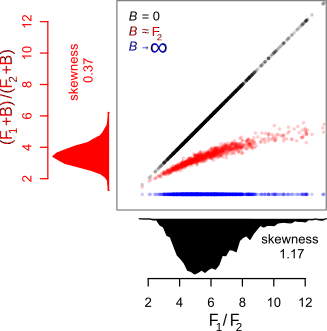
\includegraphics[width=3in]{FIGS/imaging/backgroundRatio.pdf}
  {\singlespacing 
  \caption[ Idiosyncratic effects of background on ratiometric features.]
            { Ratiometric features are idiosyncratically affected by background.
            The same initial data as in the right panels of \ar{fig:imaging:SBeffects},
			but where each single-nucleus ratio
            after addition of background is plotted against its true value (1000/3700 cells shown).
            To each average was added 0 (black), 1000 (red),
            or $10^{10}$ (blue) background units before taking the ratio. The first
            two artificial cases are the same as those in \ar{fig:imaging:SBeffects}.
			The impact on the apparent ratio
            is dependent on the relative sizes of the foregrounds and the background,
            such that the data becomes scrambled in the red curve.
            Note that
			the distribution shape is also affected, such that adding background
			decreased the skewness. $F_1$, average
            single-nuclear Hoechst; $F_2$, average nuclear Smad2/3.}
  \label{fig:imaging:backgroundRatio}}
  \end{figure}


In the second case, we could allow $F_{c1}$ and $F_{c2}$ to come
from distinct channels, which would also allow them to have
different shading
and background. As a consequence, the effects on the
distribution properties are extremely difficult to predict
due to the presence of many independent variables
(as indicated in the case study in \ar{fig:imaging:SBeffects}, right panels).
I therefore leave the discussion here, with
the conclusion that the mean and variation of the ratio feature can both
increase or decrease with different ranges of component values.
This unpredictability has important
ramifications for applications such as
fluorescence resonance energy transfer (FRET) where interpretation
relies on accurate cross-channel ratios \cite{Hodgson2010}.


\subsubsection{On the importance of image correction}

Unfortunately, the mathematical discourse above leaves us
with the dissatisfying result that the importance of image correction
is highly dataset dependent. In \ar{fig:imaging:SBeffects} I show
the size of the distortion for an example dataset with
experimentally-reasonable amounts of background and shading, which
shows effects that are measurable and sometimes relatively large. However,
different analytical requirements can tolerate quite different
amounts of feature distribution distortion before
data interpretation is affected.
The best I can do then, besides the easy blanket statement
``always correct your images!'' is to provide a few rules of thumb for
deciding on the importance of image correction.


First, I
completely ignored the detector contribution ($D$) in the above
discussion because
the matrix $D$ is unchanging and is therefore trivial to subtract from
images. Removal of $D$ should be a part of all image
analysis pipelines. This step is rarely explicitly performed
in the literature but can have a large impact
on measurements of weakly-fluorescent samples. In particular,
shading will be underestimated without subtraction of the detector
fluorescence contribution.


Second, shading tends to increase feature distribution widths
and so should be corrected whenever measurement of true biological
variability is important. Additionally, if the foreground to background ratio
is low, then shading may cause foreground values in one part of an image to fall below
background values in another part. This can have
important consequences to image segmentation \arp{imaging:segmentation}
\cite{Herbert2012}. However, in the case that biological
variability is high relative to the variation in shading
it would not be necessary to correct for $S$.
This is because the observed average and total distributions are
the convolution
of the shading and foreground distributions. If two normal distributions
with variances $\sigma^2_1$ and $\sigma^2_2$ are convolved, they yield a new
distribution with $\sigma^2_3=\sigma^2_1+\sigma^2_2$. Because shading
is a relative term, we have to scale it to the size of $F_c$ to make
use of this property: $\sigma^2_{\text{observed}}=(F_c\sigma_{S_c})^2+\sigma_{F_c}^2$.
Thus, if $F_c\sigma_{S_c}^2<<\sigma_{F_c}^2$ the observed
distribution will be close to the true distribution. While this
is a useful rule of thumb, I note that I have never observed normally-distributed
shading values (see examples in \ar{fig:imaging:properties}b).


Third, background can dramatically shift feature distribution
means. Background should therefore be corrected either when accurate means
or accurate ratios between two means are needed. When background
is low compared to even the lowest foreground values, however, it will have
little impact on the feature distributions discussed above.


Finally, when using cross-channel ratios extra care should be
taken to ensure that both background and shading are corrected.
These ratios should always be interpreted with an eye towards
the possible
effects of imaging artifacts, as artifacts can distort rations
in unpredictable ways.


\subsection{Review of image correction methods}
\label{imaging:correction:review}


Now that I have given some motivation for the importance of image correction, 
I turn to the available methods for this
process. Here, I briefly review the correction methods that
are commonly employed in the literature. In general, when deciding
on a method the investigator should test its theoretical performance
given the image model described in this chapter, $I=D+S(F+B)$.
By taking this approach, deficiencies or important assumptions of
the methods should become clear.


There are many published methods for fluorescence image correction,
perhaps as many methods as there are labs, due to the idiosyncrasies
of imaging data and the lack of standardized approaches.
I group the most common methods into two broad, non-exhaustive
categories, which I refer to as ``reference-image'' and ``per-image''
correction.
Reference-image methods obtain correction parameters from one image
and then use those parameters to correct another image. Per-image methods
find such parameters in the very image that is to be corrected.


Reference-image methods are straightforward and so are commonly used and 
recommended throughout the literature
\cite{VandenDoel1998,Model2001,Zwier2004,Wolf2007,Waters2009}.
These methods make a key assumption: that the reference image 
has approximately the same shading and background
as do the images to be corrected. A good example of this approach
uses two reference images to flatten shading, subtract background,
and normalize the fluorescence
intensity to a standard \cite{Model2001}.
One reference image, $I_\text{uniform}$ contains a
dissolved fluorophore; because this image would be flat without shading, it can
be used to determine how much shading is present in the real images. The other
reference, $I_\text{background}$ is the same as the sample images but contains no
sample. This image can thus be used to estimate background.
Equations~\ref{correction:example1}\nobreakdash-\ref{correction:example2} demonstrate this method.
	%
	\begin{align}
	I_\text{sample}     &= D+S(F_\text{sample}+B) \label{correction:example1}\\
	I_\text{background} &= D+SB \label{correction:ib} \\
	I_\text{uniform}    &= D+S(B_\text{uniform}+B) \\
	I_\text{corrected}  &= \frac{ I_\text{sample}-I_\text{background} }{ I_\text{uniform}-I_\text{background} }
		= \frac{ [D+S(F_\text{sample}+B)]-[D+SB]}{ [D+S(B_\text{uniform}+B)]-[D+SB] }
		= \frac{F_\text{sample}}{B_\text{uniform}} \label{correction:example2}
	\end{align}
	


While reference-image methods are straightforward and often easy to perform,
some of those recommended in the literature are only partially corrective. This is especially
true with respect to the detector value $D$, which
I have not seen explicitly accounted for in these methods.
To find out if a given method performed complete correction, investigators can plug the
image model into the method and check that, algebraically, the output is either
$F$ or some normalized form of it (as in \ar{correction:example2}).
However, note that partial correction may be
sufficient in some cases, particularly when background intensity is low compared
to foreground intensity and when within-image shading variation
is low compared to foreground variation.


Per-image methods, on the other hand, have the challenging task of measuring
all image components ($D$, $S$, $F$, and $B$)
within the image that is to be corrected. These methods typically
work by trying to fit a model to the combination of non-foreground
layers, $D+SB$. Therefore the primary difficulty
is that images typically contain varying fractions of foreground pixels
(e.g. due to variation in cell density),
so that determination of which pixels consist of background
is non-trivial. Further, even if identification of background pixels
is straightforward within an image, the size of the background signal
``underneath'' a foreground object is necessarily unknown and must
be predicted. The method for this prediction is what separates the different
per-image correction algorithms. 


Some per-image methods fit a polynomial \cite{L2000}
or spline surface \cite{Lindblad162266,Lindblad2004,Yin2013} to predicted
non-foreground pixels, therefore assuming a 
particular structure to the shading patterns.
These methods may also assume properties of 
the foreground objects (e.g. fluorescing cells),
such as a maximum size in the case of the rolling ball algorithm employed by
ImageJ\cite{Schneider2012} and Fiji \cite{Schindelin2012},
and may perform non-linear transformations of the underlying
images. Additionally, the accuracy of these
approaches necessarily decreases with
increasing cell density as there are fewer
background pixels from which to estimate
$I_\text{background}$. High confluency or cell clumping can thus cause
per-image methods to introduce artifacts.


When they work properly, per-image based methods generate
$I_\text{background}$ \arp{correction:ib} 
from each sample image, $I_\text{sample}$ \arp{correction:example1}.
From this point, then, the reference-based and per-image based
correction methods are the same; the only difference is in how
$I_\text{background}$ is obtained.
The question that then remains in both cases is which
mathematical operation to perform in order to correct the sample images. 
In the literature,
subtraction ($I_\text{sample}-I_\text{background}$) is frequently
used. However, subtraction does not remove
shading, as the algebraic result is $SF$ instead of $F$. The standard
rolling ball algorithm employed by ImageJ and
FIJI uses this subtractive approach.


The better approach is to use division to remove shading. This can be
done in combination with subtraction to remove both background and shading,
as in the example above \arp{correction:example2}. However, many studies
use simple division ($I_\text{sample}/I_\text{background}$), which results
in $\frac{D+S(B+F)}{D+SB}=1+\frac{SF}{D+SB}$. This result is a
background-normalized foreground with incompletely-corrected shading.
The correction can be completed by prior subtraction of $D$ from both images,
followed by subtraction of 1, which would yield the normalized image $F/B$.


I use a different approach from those listed above, 
which is to independently estimate all
non-foreground parameters so that I can perform the image algebra
that expicitly returns $F$. I discuss this method next.


\subsection{An improved correction method for high-throughput imaging}
\label{imaging:correction:myMethod}


Having determined the importance of image correction, and observed
the diversity and frequent inaccuracy of the available correction methods,
I sought to develop a simple and robust method for my own imaging applications.
All of the work in this dissertation took advantage of the throughput of
microtiter plates (e.g. 96- and 384-well plates), and so in particular I needed
to be able to accurately correct large numbers of images with
minimal computational overhead.
Further, I needed the correction to be robust to cell density,
so that I could correctly measure single-cell biological variability
under a wide variety of experimental conditions.


The approach that I developed (published in \cite{Coster2014}),
is a reference-based
method that relies on a key observation: shading patterns
are highly predictable
in microtiter plates. This allows for a correction method
that forgoes the need to
estimate parameters for every image, yet is more accurate
than using only
a single set of correction parameters. Below I show the
evidence that shading is indeed predictable, and then outline
a correction method for taking advantage of this fact.


\subsubsection{The shading pattern is a function of within-well position}



  \begin{figure}[!bt]
  \centering
  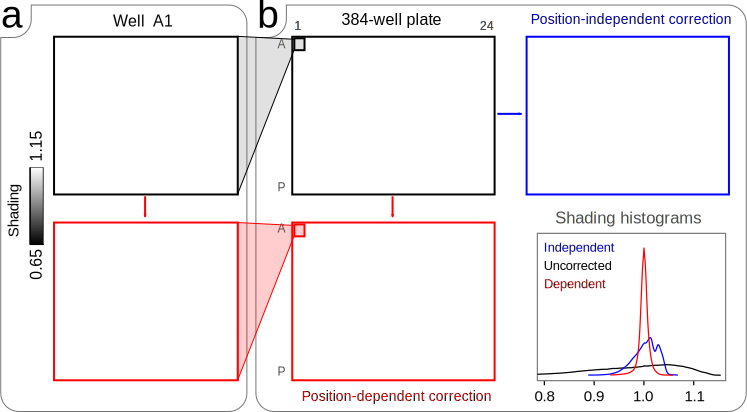
\includegraphics[width=6in]{FIGS/imaging/plateCorrection.pdf}
  {\singlespacing 
  \caption[ Demonstration of within-well positional image correction.]
            { For a within-well position, shading patterns are consistent
			throughout the entirety of a microtiter plate.
			I imaged 3x3 grids within every well of a 384-well
			plate containing dissolved fluorescein. Optical setup:
			black plastic 384-well plate (Corning \#3712), FITC filter,
			20X objective, Andor sCMOS camera.
			I cropped all images identically to remove pixels that contained
            well edges. Within-well images were montaged
			into a single image, and then normalized to the median pixel
			value of that montaged image (e.g. in \b{a}, top). This converts
			the images to an estimate of shading as defined in this chapter.
			Reference 3x3 image montages were
            made by taking the per-pixel average
			across all 3x3 montages (from all wells).
            This was done either with all 9 images in
			the 3x3 grid (Position-dependent correction) or with only the
			central image from the grid repeated 9 times
            (Position-independent correction).
			Finally, the resulting grids were montaged to show the image
			properties across the entire 384-well plate (\b{b}). Panel
			\b{a} shows larger thumbnails of the 3x3 image grids in well A1
			before and after position-dependent correction. The histograms
			in \b{b} shows the distributions of all relative pixel intensities
			in the montaged images. Tighter distributions indicate more
			accurate correction. White objects in the montaged images are
			auto-fluorescing debris; small black corners in remaining in
			corrected images are due to inclusion of a small portion
			of the black well edge.}
  \label{fig:imaging:plateCorrection}}
  \end{figure}


I was initially surprised at the high variability in shading patterns that I
observed within imaging datasets from microtiter plates.
In the literature there
appears to be an implicit assumption that such
variability is common and unpredictable,
as the most common correction methods used in big datasets are
per-image. However, shading is an artifact that is
generated by the light path, which is a static aspect of the microscope
optical setup, and so I would have expected it to be
unchanging within a dataset. Indeed, images taken at different positions along a
glass slide seem to show an unchanging shading pattern.
I therefore reasoned that it was the microtiter plates
themselves that modified the
shading pattern. Further, since microtiter plates are essentially
arrays of identical wells, I
predicted that the shading modification must be a function of the
image location
within a single well (as opposed to the position within the plate).
The source of the within-well shading modulation could be due to
reflections from well edges, local distortions
of the imaging surface, or lensing by
the solvent meniscus.


This prediction of within-well positional dependence of
shading patterns bore out, as can be seen in
\ar{fig:imaging:plateCorrection}. Further, this turned out
to be consistent for both 384- and 96-well plates from various
manufacturers and with different physical specifications
and materials. In 96-well plates
this positional effect is less dramatic, which is consistent with
shading patterns being modified by well edges (as these edges
are much further apart than are those in 384-well plates). I also note that
a position-independent correction method (that uses a single reference
image instead of one per within-well position,
\ar{fig:imaging:plateCorrection}, blue) dramatically improves
the images as well. Therefore this even simpler method may be suitable
for some datasets (though the resulting multi-modality in
\ar{fig:imaging:plateCorrection} could, in principle, generate
artificial cellular subpopulations \arp{introduction:variability}).




\subsubsection{Pipeline for within-well position-based image correction}
\label{correction:pipeline}

The within-well positional shading constancy allowed
me to implement a simple and robust image correction pipeline
for images from microtiter plates. This pipeline is based on the
existing reference-based approaches discussed above and in other
sources \cite{Bray2012,Bray2013}.




  \begin{figure}[!bt]
  \centering
  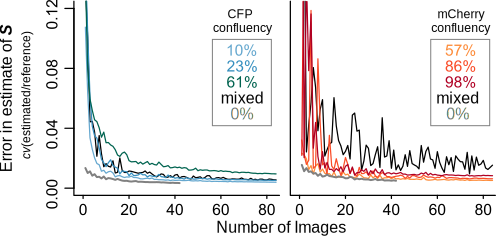
\includegraphics[width=5in]{FIGS/imaging/samplenum.pdf}
  {\singlespacing 
  \caption[ Estimating $S$ from sample-containing images.]
            { Shading ($S$) can be estimated using sample-containing
             images. Media-only wells are controls (0\% confluency).
             The spatially uniform fluorescence in these control wells was used
             to estimate the 
             ``reference'' shading by per-pixel averaging
             across 42 media-only control wells. I define
             ``confluency'' as the fraction of pixels in an image
             with intensities >3$\sigma$ above background.
             I used A549 cells expressing two differently-colored
             fluorescent proteins (left, nuclear CFP; right,
             cytosolic mCherry) at three different seeding
             densities (each seeding density had 84 replicates),
             effectively yielding six different confluency
             levels. I additionally created mixed-confluency
             image sets by randomly selecting across all
             confluency levels within each color channel.
             For each fixed number of images, $n$,
             selected from the same within-well position, I computed
             the ``estimated shading'' as the per-pixel median of
             $n$ randomly selected images. The error in the shading
             estimates are computed as the $cv$ of the per-pixel 
             ratio of (estimated shading)/(reference shading).
             For each confluency level, the inaccuracy of the
             sample-based shading estimate generally decrease
             with increasing numbers of images.}
  \label{fig:correction:samplenum}}
  \end{figure}

  

\begin{enumerate}

\item \textbf{Calibrate the microscope stage for the microtiter plate.}
Ideally, images should be acquired near well centers,
and relative within-well image positions should have
minimal drift between wells (e.g. images in well A1
should not be closer to the left well edge than those in H12).
It is important to be aware that this method will become
inaccurate with increasing positional drift. Also note that
microscope stage-driving software can vary in its accuracy,
and so custom solutions might be required for plates with
small wells.

\item \textbf{Measure the dark current component, $D$.}
The simplest approach is to capture images without a light
source, or with the light path diverted from the camera,
and per-pixel average the images. In practice, a small
number of images is sufficient ($n$=6-20 in my analyses).

\item \textbf{Subtract dark current, $D$, from all images in
the dataset.} The resulting images ($I-D$) are then modeled
by $S(B+F)$. This important step should be performed
regardless of the correction method subsequently
used, for the reasons explained above.
Without subtracting $D$, the estimated shading
patterns can become increasingly inaccurate with large
foreground values or small background values.

\item \textbf{Estimate shading $S$ for each distinct within-well
position.} This step is the most complicated in the pipeline
and should be performed with care. The goal is to obtain a
reference shading pattern for each within-well position.
For example, if an investigator has 9 images/well she will
need to estimate 9 shading patterns. There are at least two
possible approaches to this estimate.

\begin{itemize}

\item \textbf{Uniform reference images.} This approach
is the most robust, but is only possible if
there are extra wells that can be reserved solely for
acquiring reference images. In these extra wells, 
add dissolved fluorophore at the appropriate
concentration for the intended exposure time.
These wells should then be imaged along with the
other sample wells. In practice, I have found that a
small number (e.g. 6) of such uniform images is often
sufficient so long as the wells are free from fluorescing
debris. Across all wells $w$, for a given within-well
position $p$, the images $I_{w,p}$ should be per-pixel averaged
to obtain a reference image $\text{R}_p=\text{mean}_w (I_{w,p}-D)$.
Note that the per-pixel median or other quantile may
be more robust.

\item \textbf{Sample-based reference images.}
In high-throughput studies extra wells may be
unavailable for acquiring reference images.
In this case, the investigator can take advantage
of the large number of available sample images and otherwise
use the same method as for uniform reference images.
Because these sample images contain foreground, many
more values per coordinate are needed to get an
accurate estimate of shading. In \ar{fig:correction:samplenum}
I show how accuracy is dramatically affected by
the number of images used. The same figure suggests that
20-40 cell-containing images may often be sufficient, but this
is dependent on the cellular confluency of those images. 
\end{itemize}


The results of this step will be one reference image per
within-well position. As defined earlier, the shading values
should be centered on 1 to maintain the original intensity
range. Therefore once all reference images are collected
each image $\text{R}_p$ should be divided by the median
or mean of all reference image pixel values (with coordinates
$(r,c)$. The resulting shading patterns are described by
$S_p=\frac{\text{R}_p}{\text{mean}_{r,c,p} R_{r,c,p}}$


\item \textbf{Correct for the shading $S$ at each
within-well position.} To correct for shading,
every image $I_p$ should be per-pixel divided by
the corresponding shading pattern $S_p$ obtained in
the previous step: $\frac{I_p}{S_p}$. The resulting
images then contain only $B+F$.


\item \textbf{Subtract the background from each image.}
There are multiple approaches to this task.
The proper choice depends on the
particulars of the dataset, and so I illustrate two
cases here. In both cases, after subtracting background
we end up with the approximate foreground signal, $F$.

\begin{itemize}

\item \textbf{Global background subtraction.}
In some datasets, the background may vary little between
images. In this case, a global background value can be
estimated by averaging background pixels from a
representative image. Subtract this value from all pixels
in all images.

\item \textbf{Per-image background subtraction.}
In other datasets, there may be significant variability
in background from well to well. This could be due to errors
in staining or variation in exposure time. 
Background values can be estimated per image
by e.g. Otsu thresholding to automatically identify
background pixels \cite{Otsu1975}. Alternatively, a low
quantile pixel value can be taken as background
(the quantile choice is dependent on cell density).
Then, for each image, subtract its estimated
background value.


I note that, in the case of background
differences being due to something that would imply foreground
differences, such as due to exposure time or staining
variation, these per-image background estimates can be used
to normalize intensities between images. For example, to
normalize all images to some reference $B_{ref}$, determine the
normalization factor by taking its ratio with the per-image
background $B_{ref}/B_{sample}$. The image can then be multiplied by this
factor at every pixel, bringing it to the same intensity level
as the reference image. Care should be taken with this approach,
however, as it is not generally obvious when background variation
is predictive of foreground variation. 
\end{itemize}

\end{enumerate}

Note that this pipeline is only meant to remove shading $S$,
background $B$, and detector $D$ from images. What is left will
be all foreground layers, which may include various artifacts.
Further, the foreground values may vary for reasons independent
from imaging. For example, it is well established that assays
in microtiter plates can show batch, edge, row, and column effects.
These effects may non-biologically change the true values of $F$
and should thus be normalized after image correction
\cite{Malo2006,Dragiev2011,Dragiev2012,Carralot2012,Zhong2013}.

  
\subsection{Image correction quality control}

As with any data manipulation, the image correction
method outlined above should be checked to ensure
that no errors are introduced.
An obvious approach is to simply
visually inspect a subset of images, as in 
\ar{fig:imaging:flatfieldCheck}a,
though automated approaches are also feasible.


For background correction,
images should be checked to ensure that only the
background has been subtracted. This can be done
by examining background pixels. Since a perfect
subtraction will have set the centroid of the
background pixel distribution to zero, roughly half
of all post-correction background pixels should
be zero while the other background pixels take on small values.
Unfortunately, this task can be difficult to automate
for the same reason that errors may be introduced:
cell density may vary dramatically within a dataset,
complicating the automated identification of background pixels.


For shading correction, the likely artifacts will be
spatial. In other words, if there is over-correction
or under-correction,
this will cause certain regions of every image (and
the cells within those regions) to have systematically
higher or lower intensities than the global mean. This can be checked
in an automated way after cell segmentation by testing
for dependence of single-cell features on within-image
position (see an example of this approach in
\ar{fig:imaging:flatfieldCheck}b).



 \begin{figure}[!bt]
  \centering
  \includegraphics[width=6in]{FIGS/imaging/flatfieldCheck.pdf}
  {\singlespacing 
  \caption[ Quality control for image correction.]
            {Images can be over- or under-corrected, and
            therefore require quality control. \b{a},
            Visual inspection should reveal a flat background
            and a foreground that does not vary in a
            spatially predictable manner after correction. Histone H2B-Cyan
            Fluorescent Protein labeled A549 cells. Image
            courtesy Jungseog Kang (Altschuler \& Wu lab,
            UT Southwestern). \b{b},
            After segmentation and feature-extraction,
            single-cell features can be tested for within-image
            spatial dependence. Top left, a sample image of
            Smad2/3-stained human colonic epithelial cells,
            showing the radial metric of ``distance from image
            center.'' Plots show nuclear area and
            total nuclear Smad2/3 or Hoechst
            as a function of within-image radial position
            ($n$=1000/$\sim$20000 randomly-chosen cells).
            Intensities were median-normalized by well to prevent
            true experimental variation from affecting this
            test of positional phenotype dependence.
            Inset
            numeric value is the Pearson correlation coefficient
            for the two variables plotted. }
  \label{fig:imaging:flatfieldCheck}}
  \end{figure}

\section{On segmentation and single-cell features}
\label{imaging:features}


Once a dataset has been collected, and corrected as
in the previous section, the analysis begins. In general,
we want to obtain interesting properties of the foreground
layers in our images. In specific, it is nearly always the
foreground properties within individual cells that we care
about. ``Segmentation'' is the process of identifying
those cells (or intracellular objects)
and extracting them from the rest of the image.
Once cells have been segmented, properties of their pixel
values and spatial arrangement can be measured and stored
as sets of features.


Cellular segmentation is still an unsolved computer
vision problem \cite{Danuser2011},
in large part because experimental needs are too specific
to allow for a good general solution. There is, however,
an array of partial solutions available. These range from simple
to highly complex, and vary tremendously in their accuracy
and utility.
In this section I briefly discuss segmentation algorithms
and how one can go about choosing single-cell
features that are biologically meaningful.
My goal in part is to provide
the rationale for my own choices for the
experimental work in \ar{insulation:introduction}.


\subsection{Segmentation approaches}
\label{imaging:segmentation}

There are many approaches to cellular segmentation.
Software solutions such as CellProfiler \cite{Carpenter2006}
implement many of the most-used segmentation algorithms
so that the user can choose one appropriate to the experiment.
Unfortunately, which algorithm should be chosen is not a trivial matter.
Many of these algorithms are complex and therefore difficult
to understand and use. Further, the simpler algorithms may fail
to provide sufficiently accurate segmentation for some image properties.
As a consequence the path of least resistance is often manual segmentation
using tools such as ImageJ \cite{Schneider2012},
but this labor-intensive approach limits the resulting sample
size and may yield biased investigator-specific outcomes.


The value of automated segmentation approaches should be obvious:
they allow for the rapid and reproducible
identification of huge numbers of cells. Automated approaches are
also biased, due to the choice of parameters for the algorithm, but
the bias is systematic and does not change between images.
There are plenty of difficulties with automation, however. With
huge datasets comes the inability to perform thorough quality
control. Additonally, there may be no single set of segmentation parameters,
or even a single algorithm, that will successfully segment all
cellular phenotypes in a diverse experimental setup (e.g. a
drug screen). Automation thus requires extensive testing and
a wary mindset.


As a consequence of these issues, I strongly advocate for use of the simplest
segmentation method that is capable of answer a given
experimental question. Because so many aspects of images
can be measured, it is easy to get carried away with trying to
obtain every single piece of data that the images contain. As already noted, however,
the number of potential measurements is large;
obtaining all data from images is not only impossible, it probably
is not wise since each extracted feature should be understood at a
biological level before it is used (and, as I discuss below, biological
interpretation of features is not a trivial task).
The use of simpler methods makes the resulting segmentation more 
understandable, and so conditions that will cause the algorithm
to produce garbage are more predictable and intuitive. A few of
the more straight-forward and commonly-used methods are
threshold, watershed, and voronoi segmentation, discussed next
(these are depicted graphically in \ar{fig:imaging:segmentationMethods}).


  \begin{figure}[!bt]
  \centering
  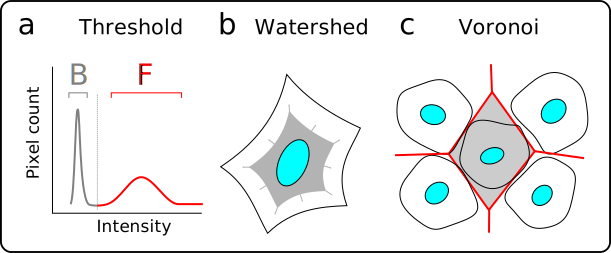
\includegraphics[width=4in]{FIGS/imaging/segmentationMethods.pdf}
  {\singlespacing 
  \caption[ Cartoon of segmentation methods.]
            {Cartoons of three basic segmentation
            methods. \b{a}, Threshold segmentation separates
            background $B$ from foreground $F$ by fluorescence
            intensity. Neighboring pixels are then considered
            part of the same object. The histogram
            represents the distribution of
            all pixel intensities within an image.
            \b{b}, Watershed starts with a known
            intracellular point (e.g. the nucleus, blue)
            and moves outwards (gray, arrows) until it reaches
            cell boundaries. \b{c} Voronoi segmentation assigns
            to a set of already-known objects all of the space closer to
            that object than any other. Red lines, boundaries
            of the Voronoi cells,
            using nuclei centroids as the known points. Gray area,
            segmented region for the middle cell.}
  \label{fig:imaging:segmentationMethods}}
  \end{figure}
  
  
Threshold segmentation (the approach that I use in this
dissertation) is probably the simplest method after manual
segmentation. It works by assuming that the pixel intensities
within cells are generally higher then those in the image
background \ar{fig:imaging:segmentationMethods}a.
Therefore a threshold can be chosen either manually
or via some mathematical or algorithmic approach (e.g.
Otsu thresholding \cite{Otsu1975}) that best separates
background and foreground pixels. Neighboring pixels classified
as foreground can be grouped into
objects, such as nuclei. This method tends to fail for whole-cell
segmentation when
cellular density is high, as neighboring cells can be segmented
as single objects. Additionally, it is not necessarily true
that the nuclear or cytosolic compartments contain higher
pixel intensities than do the background. This is dependent
on the probes used, and is of particular difficulty for
live-cell imaging (see Appendix \ar{pseg} for an experimental solution).
Cellular nuclei are frequently
segmented using this method, as they tend to be spatially distinct
even with high cell density, and DNA stains such as Hoechst
and DAPI create bright foreground signals. Threshold-segmented
nuclei often form the basis for more complex algorithms.


There are many specific algorithms for watershed segmentation
\cite{Vincent1991,Malpica1997,Loo2010} but the general
approach is roughly the same. The algorithm starts with
a ``seed,'' which is a pixel coordinate in the image.
This seed can be randomly generated or chosen from centroids
of threshold-segmented nuclei. The algorithm then searches
away from that seed point, following paths of increasing
intensity (\ar{fig:imaging:segmentationMethods}b).
Sharp decreases in intensity, as frequently
occurs between cells or between a cell edge and the background,
will cause the outward movement to stop. These algorithms
are thus useful for segmenting irregularly-shaped and slightly
crowded cytosolic regions. However, they may require many parameters, and
can yield over-segmentation (the breaking up of single cells
into many objects).


The final method that I want to make note of is Voronoi
segmentation. I have not frequently seen this method used in
the context of segmenting cells in tissue culture, but it
can be useful in the case that cells are at an extremely
high density (so that there is no background) and when
those cells are similar in size and relatively round
or cuboidal. With this approach,
a set of seeds are again needed. These will typically be
the centroids of threshold-segmented nuclei. For each centroid,
then, the algorithm assigns to it all space closer to that centroid
than to any other (\ar{fig:imaging:segmentationMethods}c).
This is a simple and efficient method for roughly segmenting
cellular cytosolic compartments.


With this brief overview of few segmentation methods, a
few points should be clear. First, many segmentation
approaches are fluorescence-based (though some use
brightfield) and so require staining of the cellular
compartments to be segmented (see Appendix \ar{pseg} for a live-cell
solution to this). Second, nuclei are much simpler
to segment than cytosolic regions, because nuclei typically
have narrower ranges of size, shape, and staining intensity.
Therefore threshold segmentation of
nuclei is generally considered to be accurate, and is
a frequent first-step for more complicated segmentation
pipelines. Third, different foreground objects may
require different algorithms for accurate segmentation.
Taken together, the above points help to explain why cellular
segmentation does not have a general solution.



\subsection{Understanding and choosing single-cell features}

Given the nearly unlimited set of features to choose from
it can be difficult to determine the subset that is most
appropriate to the study at hand. There are a few broad
approaches to this problem. The obvious, but non-trivial, approach is to
first choose the biological property of interest and then
identify or create features that approximate that property.
A less obvious approach is to obtain a large number of
features and use computational methods to choose those that
are the most informative \cite{Singh2010}.
In the latter case, the features need
not be biologically interpretable at all. For this discussion
I focus on the first case.


Biologically-motivated features are necessarily approximations
of the underlying property of interest. It is therefore important
to be aware of how the features are defined so that the data
can be interpreted properly. As an example, a project in the
Altschuler \& Wu lab required measurement of neutrophil polarity, but
needed that measurement to be performed on fluorescently-labeled
cytoskeletal components. There is no obvious mathematical
feature of fluorescently-labeled actin or microtubules that would indicate the
degree of polarization of a neutrophil. An approximate solution was
therefore developed, which measures how close together in space are the brightest
pixels \cite{Ku2010,Ku2012}.


This polarity feature will decrease in value with, for example, 
increased collection of actin to one side of the cell.
In the case that the actin intensity is diffuse throughout
the cell, the brightest pixels will also be
diffuse and so the feature value increases.
This feature therefore serves as a useful proxy for polarity. However,
the feature is sensitive to bright punctate artifacts that
are common to immunostained images and is distorted by differences in
cell size. By being aware of these pitfalls they can
be addressed. In this case, visual quality control was performed
on every cell to ensure
the absence of artifacts, and the feature calculation was modified to compensate
for distortions due to cell size \cite{Ku2010,Ku2012}.


Investigators will more frequently use combinations of
simpler features, such as those describing aspects of cell
size and shape (``morphological features'') and
of fluorescence intensity (``intensity features''). It is
important to be aware that these two classes are not completely
independennt. Intensity features in particular can be highly
dependent on morphological features.


As a simple example,
the average intensity is dependent on the area.
It is therefore important to interpret changes to the average
with care, as the change could result from  a
change in cell size, a change in concentration of the labeled
protein, or a combination of the two.
The ratio of nuclear to cytosolic average intensities
additionally suffers from this potential confusion. It has
an added difficulty, however, in that a change in the ratio
can be due to movement of the labeled protein from one compartment
to the other, or to independent changes in one or both compartments.


Ideally, then, a
feature should be carefully chosen to have an unambiguous biological
interpretation and be independent of
other features whose changes are not important to
the study. I argue that interpretability is more important than having
a feature that more closely approximates the biological property
of interest. For example, in my own work (\ar{insulation:introduction})
I am interested in the
concentrations of nuclear transcription factors. Concentration
is intuitively approximated by the average intensity feature, yet
I instead chose the total intensity feature for all of my analysis.
I did so because certain properties of the total intensity feature,
discussed next, allow for less ambiguity in how to interpret
changes in its values.


\subsection{Benefits of the total nuclear intensity feature}
\label{imaging:totalIntensity}


The total intensity
feature is a proxy for the absolute count
of a fluorescently-labeled target molecule. This feature has the
advantage of being independent of cell size, such that changes
in cell morphology may change the average but not total
intensity. Unfortunately, intensity from widefield microscopy images
does not just come from the focal plane, but also from the
space both above and below that plane. As a consequence,
in image represents a messy volumetric cross section through the $z$-axis.
This fact adds some complication to the interpretation of the
total intensity feature: is it measuring the total number of
molecules in the entire cell volume, from a thin cross-section,
or something in between?


Fortunately, my focus on transcription factors in 
\ar{insulation:introduction} allows me to mitigate this concern
by measuring only the nuclear intensities. The nucleus
tends to maintain a taller stature in the $z$-axis than does
the rest of the cell (resulting in the famous ``fried egg'' appearance
of cells in tissue culture). Also, nuclei tend to be of
more similar size and shape than do cytosolic compartments.
For these reasons, I can reasonably assume that whatever the
thickness of the imaged section, I will be imaging a similar
thickness for all nuclei.


Finally, and perhaps most importantly, the nucleus
has a built-in ``ground truth'' for this feature that allows
for both quality control and removal of measurement error
\arp{imaging:variation}.
This ground truth comes from the DNA content of cells, as
each cell within e.g. the G1 phase of the cell cycle in reality
has a near-identical total DNA content. The total intensity
feature is a proxy for this content. Importantly,
total nuclear intensity is the only feature
with such a ``ground truth'' reference.
The small-molecule stain Hoechst
provides a robust and DNA-specific signal that I use throughout
this dissertation to measure total DNA content. I therefore use
the term ``DNA'' interchangeably to refer to the actual molecule
and as a short-hand for ``Hoechst-stained DNA.'' 


\subsection{Measuring information content of a feature}
\label{imaging:information}

One of the major hurdles in experimental cell biology
is our lack of initial knowledge about which environmental
signals ($S$) and cellular responses ($R$) cells care about
(discussed in \ar{introduction:introduction}).
As a consequence, it is generally unclear how
much information about the environment a cell can accurately process
and store, though estimates suggest that the features
we believe cells care about contain
somewhat unimpressive information content \cite{Cheong2011}.

  \begin{figure}[!bt]
  \centering
  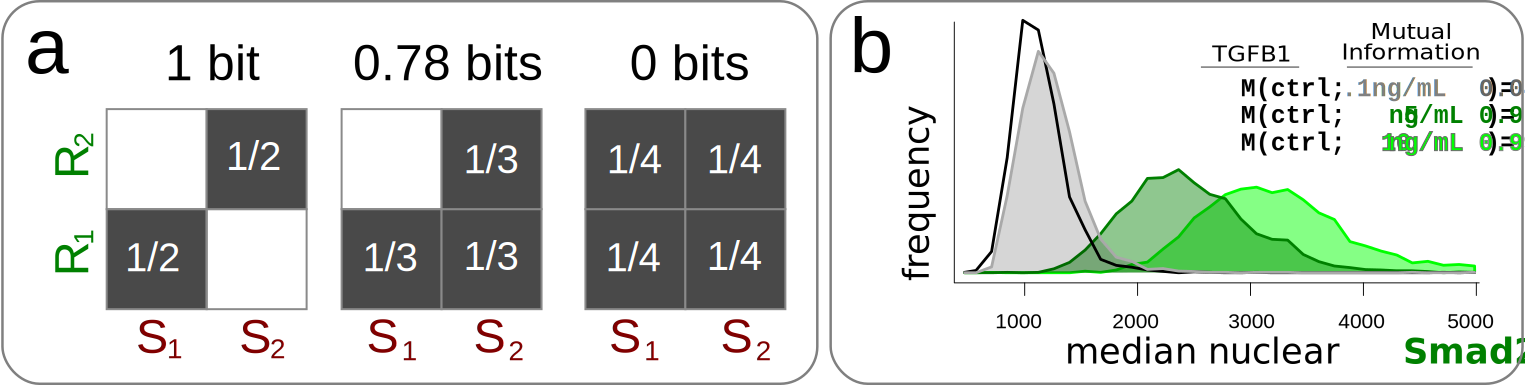
\includegraphics[width=6in]{FIGS/imaging/MI.pdf}
  {\singlespacing 
  \caption[ Mutual information examples.]
            {The mutual information metric can be interpreted
            as yielding $\log_2$ of the number of distinct signal-response
            relationships. \b{a}, A toy cases with
            only two signals, $S_1$ and $S_2$, and two responses,
            $R_1$ and $R_2$, with uniform joint probabilities. Darkened
            boxes show occurring signal-response relationships and their
            joint probabilities. Left, two completely distinct
            signal-response pairs yield $\log_2(2)=1$ bit of mutual
            information. Middle, both signals cause response $R_1$,
            meaning that observation of $R_1$ provides insufficient
            information to know which signal caused that response. The mutual
            information thus decreases to $\log_2(81/16)\approx0.78$
            bits (using \ar{eq:imaging:mi}). Right, with both signals
            causing both responses with equal probability, there is
            no mutual information ($\log_2(1)=0$ bits).
            \b{b}, Mutual information measurements of TGFB1-Smad2/3
            responses. Distributions show the wide variability
            of nuclear Smad2/3 accumulation even in response to
            saturating (10ng/mL) ligand concentrations. Observe
            that the control and saturating doses yield distributions
            that are nearly non-overlapping, and as a consequence
            yield $\sim$1 bit of mutual information (as there are 2
            distinct signal-response relatinships). It should be clear
            that the mutual information between all concentrations and
            outputs can be calculated at once, but there is significant
            overlap between all but the outermost distributions. Thus,
            addition of each subsequent intervening signal will in this
            case yield diminishing improvements to the mutual information
            between TGFB1 and nuclear Smad2/3.
            $n$>3000
            human colonic epithelial cells per condition. I used
            an implementation of the mutual information algorithm as described
            in \cite{Cheong2011}.}
  \label{fig:imaging:MI}}
  \end{figure}

Measuring the information content of a feature with
respect to the signal under study can therefore be useful
when trying to choose between a set of potential $(S,R)$
combinations. This can be
done using the ``mutual information'' metric
between the signal and response, $M(S;R)$  \cite{Cheong2011}.
Mutual information has advantages over other statistical metrics,
such as Z-scores and the like, in that it is completely
non-parametric (i.e. does not assume a distribution shape)
and uses units that
can be directly interpreted as ``information content,'' measured in bits.
I use this metric in \ar{insulation:introduction} to compare
the information content of ligand concentrations for \tgfbsf\
and Wnt, and so here I dig into mutual information a bit
deeper\footnote{Did you catch the joke?}
with the goal of providing an intuition to the reader
regarding its interpretation.


The mutual information between a set of signals $S$
(e.g. ligand concentrations) and
responses $R$ (e.g. nuclear transcription factor concentrations) is defined
by \ar{eq:imaging:mi}. In the formula, $P(R,S)$ is the joint
probability of each signal-response pair
and $P(R)$ and $P(S)$ are the marginal
probabilities.
The mutual information value returned by this formula
is in units of ``bits,'' and can
be interpreted as the $\log_2$ of the number of
distinct signal-response relationships
(see \ar{fig:imaging:MI}a for a toy example).
In essence the quantity describes how accurately
we would be able to guess the signal if we were
told the response (and vice versa).
The goal of the mutual information metric then
is to measure the degree of overlap between
signal-response distributions, it is not to measure
how far apart those distributions are. For example,
two completely separated response distributions will
always have 1 bit of mutual information even if they
are infinitely far apart. Therefore the maximum possible
information content is $\log_2$ of the number of distinct
signals (\ar{fig:imaging:MI}a, left). The minimum mutual information is zero, which
occurs when the distributions completely overlap (\ar{fig:imaging:MI}a, right).
    %
    \begin{equation} \label{eq:imaging:mi}
    M(R;S)=\sum_S\sum_R P(R,S)\log_2\left(\frac{P(R,S)}{P(R)P(S)}\right)
    \end{equation}



Importantly, single-cell
variability in nuclear transcription factor
concentrations is high, such that even the
untreated and saturating ligand
doses yield a small overlap in cellular
responses (\ar{fig:imaging:MI}b) \cite{Cheong2011}. In other words,
if we were given a randomly drawn cellular Smad2/3
response from a dose-response curve for TGFB1 treatment,
we would have high uncertainty as to the precise
TGFB1 concentration that caused the drawn response.


In summary, mutual information is a metric that
measures the overlap of distributions, and so can
be interpreted to indicate the number of distinct
signal-response pairs for a given feature. This
metric can thus be used to directly measure the
relative information content of different features $R$
or signals $S$ (as I do in \ar{insulation:system}).

\section{Dealing with variation}
\label{imaging:variation}


Experimental error is always present in our
measurements. Additionally, any given feature
may show extensive biological variability even within
apparently homogeneous populations. The biological
variation can be informative, as it gives us
insight into the limits to accuracy of cellular
processing and can reveal phenotypically distinct
subpopulations (see \ar{insulation:introduction}).
However, if experimental error is mis-interpreted
as biological variability, we lose statistical resolution
or may assign unwarranted meaning to non-biological
variation. It is then important to be able to separate
experimental from biological variation.


Experimental variation in fluorescence imaging
comes from many sources.
The imaging plane itself may cause
variation by intersecting cells at different
relative heights. This focal plane effect
can cause cell-to-cell differences in the
degree of focus and in how much off-plane
fluorescence is captured. As discussed
in \ar{imaging:distortion}, image shading and
background can also contribute to artificial variation
due to microscopy.


Aside from microscopy artifacts, the process
of preparing cells for imaging may also
generate distortions of true biological variability.
For example, variation in cellular surface
area or volume may lead to differences
in how well an antibody or non-permeable dye
can access an intracellular target.
Such differences in cell morphology may be
enhanced or dampened by fixatives, which can cause cells to shrink
in the $z$-axis \cite{Pawly2006}.


  \begin{figure}[!bt]
  \centering
  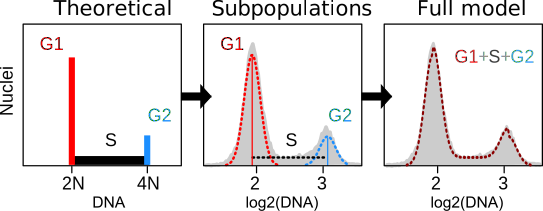
\includegraphics[width=4in]{FIGS/imaging/cycleFit.pdf}
  {\singlespacing 
  \caption[ Fitting total DNA to a simple cell cycle model.]
            {An asynchronous cell population can be
            fit to a simple model of the cell cycle
            with reasonable accuracy. Left,
            the theoretical
            asynchronous cell-cycle distribution consists
            of delta functions for G1 and G2 cells (i.e.
            all cells in these populations have identical
            DNA content) and a uniform distribution for
            S-phase cells that are moving from the G1 to G2
            states at a constant rate. Middle, the
            total DNA feature of G1 and G2 nuclei shows log-normal variation
            that can thus be fit to normal distributions after log-transformation.
            Right, the cell subpopulation models 
            add up to a reasonably accurate estimate
            of the cell cycle distribution. Gray, filled
            histograms are of $\log_2$(total DNA), with 
            DNA in arbitrary units, of $\sim2\times10^4$ Hoechst-stained
            human colonic epithelial cells. Dashed lines are
            the actual fits to this data using the method described
            in the text.}
  \label{fig:imaging:cycleFit}}
  \end{figure}


Finally, non-biological variation can be introduced
during segmentation. This can be due to outright errors
(e.g. a cell being split into two objects) or to
the more subtle fact that the accuracy of a set of
segmentation parameters will vary from cell to cell.
For example, a chosen threshold that perfectly separates
background from foreground for one cell may end up
discarding the outer edges of a dimmer cell.


\subsection{Using DNA features for quality control}
\label{imaging:variation:dnaQC}

Due to the error sources discussed above (among others)
there may be many outlier cells to discard. Manual or pseudo-manual
approaches are often used for this task. 
Visual inspection of a random
subset of segmented cells is a common approach,
though automated solutions are needed for large datasets.
An example is the identification of out-of-focus images using
image-level features from tools like PhenoRipper
\cite{Rajaram2012}.
I use an automated statistical approach that takes
advantage of ``ground truth'' aspects of total DNA
content in cells. 
This approach uses population-level statistics
of DNA features to determine which cells
are likely to be properly
segmented and in focus. In effect, I make the assumption that
cells with biologically-unlikely DNA feature values will have
non-biological values in other features as well.




  \begin{figure}[!bt]
  \centering
  \includegraphics[width=6in]{FIGS/imaging/qualityControl.pdf}
  {\singlespacing 
  \caption[ Using DNA features for quality control.]
            {DNA features can be used for single-cell quality
            control. Bottom left, the Total DNA feature
            is fit to a cell cycle plot (fit not shown)
            and the G1 population is gated as all cells
            within $\mu_{G1}\pm2\sigma_{G1}$ (blue). The population is
            also statistically gated using the nuclear area (bottom,
            middle) and the intra-nuclear intensity $cv$ (bottom, right).
            The gating is $\pm3\times\text{MAD}$ from the median of each
            feature, where $\text{MAD}$ is the median absolute deviation
            ($\text{median}(|X-\text{median}(X)|)$. 
            ($3\times\text{MAD}\approx2\sigma$ for normal distributions.)
            The gated points are considered to be in-focus G1 cells
            that are likely segmented properly. In the top plot,
            these quality-controlled
            cells are found as red points within the blue box. Data from
            >4000 Hoechst-stained human colonic epithelial cells.}
  \label{fig:imaging:qualityControl}}
  \end{figure}



The first step in my quality control pipeline is to identify cell cycle
subpopulations by fitting a cell cycle model
to the total DNA histograms. This allows for later isolation
of these subpopulations and removal of outliers. Note that
in tissue culture microscopy
mitotic (M-phase) cells are often lost during sample washes
and so are already excluded from analysis.


An asynchronous cell population can be accurately
fit to a simple model of the cell cycle. The
theoretical, variation-free model of this cell cycle
consists of of delta functions for the G1 and G2 peaks
with a uniform S-phase distribution in between
(\ar{fig:imaging:cycleFit}, left). In other words, all
cells within G1 or G2 have the exact same DNA content,
and cells moving through S-phase increase their DNA content
at a constant rate. In reality,
the cell cycle distribution arising from measured
total DNA consists of $\log$-normally distributed G1
and G2 peaks, with a variable-shaped S-phase distribution
in between. I note that, on a $\log$-scale, the G1 and
G2 distributions have near-identical standard deviations
($\sigma_{G1}\approx\sigma_{G2}$).



I implemented a simple variant of the
Dean-Jett-Fox cell cycle model \cite{Dean1974,Fox1980}
that is sufficient to accurately identify G1 and G2 cells
from microscopy data.
The formulae that comprise this model are in
Equations~\ref{eq:imaging:g1}\nobreakdash-\ref{eq:imaging:g2},
where: $T_c$ is the $\log_2$-transformed
total DNA of a single cell; $\mu_{G1}$ is the average of this
value across all G1-phase cells; $\sigma$ is the standard
deviation of the G1 and G2 distributions; $v$ is the height of the S-phase
uniform distribution, $f(T_c)$ is the fraction of
cells with the same $T_c$ DNA content (in practice, it is the fraction of cells
falling into the same histogram bin), and $w$ values are weights. \ar{fig:imaging:cycleFit} shows
this model graphically, fit to experimental data.
    %
    \begin{align}
    f_{G1}(T_c) &= \frac{w_1}{\sigma \sqrt{2\pi}}
    e^{-\frac{(T_c-\mu_{G1})^2}{2\sigma^2}} \label{eq:imaging:g1}\\
    f_{S} (T_c) &= \left\{
        \begin{array}{lr}
        0 & : T_c \notin [ \mu_{G1}, \mu_{G2} ] \\
        v & : T_c \in    [ \mu_{G1}, \mu_{G2} ]
        \end{array}
        \right.
    \label{eq:imaging:s}\\
    f_{G2}(T_c) &= \frac{w_2}{\sigma \sqrt{2\pi}}
    e^{-\frac{(T_c-\mu_{G2})^2}{2\sigma^2}} \label{eq:imaging:g2}
    \end{align}


While fitting to a cell cycle distribution model may
be sufficient to identify biological outlier cells, I use two
additional DNA features to further exclude low-quality
images of nuclei. These features
are the nuclear area and the coefficient of variation ($cv$)
of intra-nuclear DNA intensity.
The $cv$ is a rough proxy for the DNA texture,
and so can be used to identify out-of-focus cells
(lower $cv$) or those with chromatin condensation or
punctate artifacts (higher $cv$). I therefore statistically
gate the population by rejecting those cells that are too
far from the median of either of these features
(see \ar{fig:imaging:qualityControl}).


Finally, I restrict my analyses to cells in the G1 phase
\arp{fig:imaging:qualityControl}.
The rationale for this is that I do not expect G1
and G2 cells to have different qualitative behaviors
for the signaling pathways that I study in \ar{insulation:introduction},
though I do expect them to have somewhat different quantitative
behaviors. The effect of combining these subpopulations
would then be a meaningless increase in apparent signaling variability.
I therefore chose the G1 population as it is
typically more populated and is less prone to
double-segmentation errors.


\subsection{Using DNA features to correct measurement error}


By using DNA features for quality control, we can thus collect
all cells within the G1 and/or G2 populations that are high-quality
(from an imaging standpoint) and accurately segmented.
The quality control described above may be a sufficient level of
data clean-up for some experimental goals, but
it does not deal with the problem
identified at the top of this section: 
that is, the separation of true biological variation from
measurement error. In other words, quality control only discards
cells that are too far from the ``typical'' cell, it does nothing
to determine or correct the measurement error in those cells that are kept.


To identify biological variability, then,
I again take advantage of the cell cycle ``ground truth.''
As shown in \ar{fig:imaging:cycleFit}, the theoretical
cell cycle distribution has no variation in the G1 or G2
populations, as all cells have exactly the same diploid
or tetraploid DNA content. The observed variation
around the theoretical values then do not carry any biological
meaning. (Note that this approximation becomes less accurate
with chromosomally-unstable cell populations.)


\subsubsection{Single-cell measurement error correction}
\label{imaging:singleCellCorrection}

If the variation in total DNA carries no biological
information, then it should not be predictive of
of other feature values: any feature dependence on
the DNA content must then be due to a global source
of error. In principle, then, we can then reduce this error by 
removing the meaningless correlations of other features to total DNA content. 


  \begin{figure}[!bt]
  \centering
  
\includegraphics[width=6in]{FIGS/imaging/singleCellNorm.pdf}
  {\singlespacing 
  \caption[ Single-cell correction using DNA features.]
            {The variation in total DNA content (within a single cell cycle peak)
            is non-biological and therefore should not be predictive of
            intensity values for other probes.
            \b{a}, Total Smad as a function of
            total DNA. The raw data show a low
            Pearson correlation coefficient (inset $r$ value)
            and linear regression slope (black line),
            which is over-corrected by
            multiplicative normalization (middle) and
            corrected by regression-based normalization
            (right). \b{b}, Comparison of single-cell values
            before (x-axis) and after (y-axis) regresson-based
            correction. This dataset has low correlation to
            total DNA, and so the change is small. 
            $n=689$ human colonic epithelial cells (G1 only,
            quality-controlled) immunostained
            with anti-Smad2/3 (Smad) and Hoechst (DNA).
            All $y$-axes on the same scale.}
  \label{fig:imaging:singleCellNorm}}
  \end{figure}

I take two single-cell level approaches to correcting
total intensity feature errors
\arp{fig:imaging:singleCellNorm}. The intuitive method
is to estimate a normalization factor for e.g. all G1 cells
using total DNA ($T_{\text{DNA},c}$), and then use this
factor to normalize the total intensity of other
fluorescent probes ($T_{\text{probe},c}$)
in those same cells (\ar{eq:imaging:dnaNorm}). Indeed,
I have seen this approach used in the literature even
without first restricting analysis to one cell cycle
subpopulation. This
method assumes a simple multiplicative relationship
between the DNA and other channels such that, for example, a 10\%
increase in total DNA content would predict a 10\%
increase in different total probe intensity. Note
that this assumption may not hold true, such that this
method can cause over- or under-correction (as in
\ref{fig:imaging:singleCellNorm}a, middle).
    %
    \begin{equation} \label{eq:imaging:dnaNorm}
    f_{\text{norm}}(T_{\text{probe},c})=
    \frac{\text{median}_c(T_{\text{DNA},c})}{T_{\text{DNA},c}}T_{\text{probe},c}
    \end{equation}

    
My preferred method is regression-based, as it
guarantees removal of
correlation between total Hoechst and the total intensity of
another probe (\ar{fig:imaging:singleCellNorm}a, right).
For this method, linear regression is performed to get the
function in \ar{eq:imaging:reg} with slope $m$ and intercept $b$.
This results in a residual value ($\text{r}_{\text{probe},c}$)
for every cell.
The value of each $T_{\text{probe},c}$ can then be corrected
by setting it equal to the median across all values plus the residual
value for the same cell (\ar{eq:imaging:regNorm}).
    %
    \begin{gather}
    T_{\text{probe},c}=f_\text{regression}(T_{\text{DNA},c})=mT_{\text{DNA},c}+\text{r}_{\text{probe},c}+b
        \label{eq:imaging:reg}\\
    f_\text{norm}(T_{\text{probe},c}) =
        \text{median}_c(T_{\text{probe},c})+\text{r}_{\text{probe},c}
        \label{eq:imaging:regNorm}
    \end{gather}

    
For the sample data in \ar{fig:imaging:singleCellNorm} it is
clear that there is low basal correlation between total DNA
and total Smad, though I have observed much
higher correlations in some datasets. I further note that this same rationale
could be extended to non-DNA references and other features
for cases in which cross-probe
correlations are expected to be meaningless.
For all datasets in this dissertation I
apply the total DNA regression-based correction when accurate
single-cell values are needed (such as for the calculation of mutual
information between single-cell distributions).


\subsubsection{Population-level error correction}


While the single-cell correction above can be used to remove
those measurement errors that are directly shared by each probe,
it is reasonable to expect that much
of measurement error is more random and so affects probes independently. Though it is
not possible to correct single-cell values for such
unpredictable error, we can apply correction at the
population level.


  \begin{figure}[!bt]
  \centering
  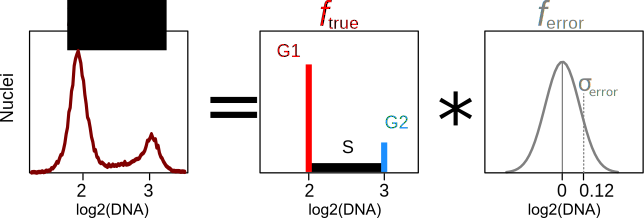
\includegraphics[width=4in]{FIGS/imaging/convolution.pdf}
  {\singlespacing 
  \caption[ Estimating measurement error of the total intensity feature.]
            {An observed total intensity distribution $f_\text{observed}$
            is the result of convolution of the true distribution
            $f_\text{true}$ and the measurement error $f_\text{error}$.
            The error function for total nuclear intensity features
            can be estimated as having $\sigma_\text{error}\approx
            \sigma_\text{DNA}$.
            Cartoon, using distributions from \ar{fig:imaging:cycleFit}.}
  \label{fig:imaging:convolution}}
  \end{figure}


An observed feature distribution can be modeled as the convolution
of a true biological distribution with a measurement error
distribution centered on zero, $f_{true}*f_{error}$. In the case of $\log$-total DNA
in G1 cells, $f_{true}$
is a delta distribution, $\delta_{true}$, positioned at $\mu_{G1}$.
I can then take advantage of
the property that $\delta_{true}*f_{error}=f_{error}+\mu_{G1}$.
In other words, the G1 and G2 distributions are themselves
estimates of the measurement error distribution, if their
means are set to 0
\arp{fig:imaging:convolution}.


For distributions that are log-normal, as are the total
intensity features for all probes used in this dissertation,
I can also use the property that two convolved normal distributions
yield a third normal distribution with mean
$\mu_3=\mu_1+\mu_2$ and variance
$\sigma_3^2=\sigma_1^2+\sigma_2^2$.
Thus, I can estimate the ``true'' cell-to-cell
total nuclear intensity variation
for any probe by \ar{eq:imaging:decon}. There of course may
be other sources of error not compensated for in this way, and
such an approach is only defensible for the total intensity feature.
    %
    \begin{equation} \label{eq:imaging:decon}
    \sigma_\text{probe,true} = \sqrt{ \sigma_\text{probe,observed}^2-\sigma_\text{DNA,error}^2 }
    \end{equation}

    
What utility does this deconvolution have? Published
measurements of cell-to-cell
variability range from 15-30\% \cite{Sigal2006a},
and my own raw data show values within
this same range. However, these values include measurement error
that is not being compensated for. Thus,
cell-to-cell variability, as measured by microscopy, is
necessarily overestimated. The above reasoning shows that
this overestimation is simple to measure, as all that is
needed are the log-scale standard deviations of the G1/2
total DNA distributions and the standard deviations of
the total-probe values in question.


I have not performed a comprehensive
study of the size of this effect, though I have measured it
in several independent datasets for various markers. I find
that deconvolved total intensity distributions yield
$\sim10\%$ lower standard deviations and $\sim10\%$ higher
information content (measured by mutual information \cite{Cheong2011}).
These inaccuracies are small enough that I feel comfortable
stating that measurement errors in high-quality microscopy datasets
are much smaller
than true biological variation.


It is important to note
that this DNA-based deconvolution makes the assumption
that the sources of error are the same between Hoechst and other probes. It is
possible that nuclear antibody-based stains have a partially non-overlapping
set of error sources with small molecules like Hoechst.
One possibility to address this, then, would be to use a
non-specific secondary antibody in a free channel.
That non-specific antibody should
not be correlated with the specific antibody staining in other
channels, and so any measured correlations could be removed using the
same rationale as for DNA content-based correction. Unfortunately,
I have had limited success with this
approach, though non-specific secondary antibodies
do indeed show high single-cell correlation. The problem has been that they also
show unexpected properties, like differences in intracellular
localization, for which adequate controls are not clear.



\section{Discussion}
\label{imaging:discussion}

Unlike other quantitative single-cell
methods, such as flow cytometry, the subcellular resolution of
image data allows for a stupefyingly
large number of feature measurements, and there are no standardized
practices for choosing or implementing these
features. Further, identification of individual
cells takes place at the level of software, not
hardware. Quantitative imaging is thus an
exceedingly difficult task outside of the labs
that specialize in it, and no two of these labs
are likely to converge on the exact same solutions.


With imaging we can directly see the beauty of the
biology we are studying, and the high information
content of images makes this type of data boundless
in its potential utility. We are currently not
meeting this potential, however, and I firmly believe
that this is due to an absence of established standards
and approaches that would make quantitative imaging more broadly accessible
and interpretable. To that end, I hope that this chapter
provides some intuition to those scientists who have
not had the opportunity to work and think extensively
about image data. Further, I hope that my approach
to single-cell image analysis, described in this chapter
and demonstrated in \ar{insulation:introduction} for
a specific biological study, provide useful demonstrations of the utility
of quantitative single-cell analysis.




\section{Methods}
\label{imaging:methods}

This chapter provides the imaging and image analysis details
also
used for the experiments in \ar{insulation:introduction}.
The methods for cell culture, immunostaining,
and imaging are left to that chapter (see \ar{insulation:methods}).
Specific methodological details for the figures in
this chapter are primarily provided within the figure
legends; this section provides the remaining information.


\textbf{Cell culture.} I followed the methods in
\ar{insulation:methods}, with the following additions.
For \ar{fig:correction:samplenum}, I used a fluorescently-labeled
clone of the cell line A549 (ATCC \#CCL-185). This clone
contains a pSeg vector that co-expresses
Cyan Fluorescent Protein fused to
Drosophila Histone H2B to label nuclei and the
Red Fluorescent Protein variant mCherry to label the whole cell
(see Appendix \ar{pseg}). The clone was generated by
Jungseog Kang and Qi Wu (Altschuler \& Wu lab, UT Southwestern).


\textbf{Imaging.} Plates were imaged on one
of two Nikon Eclipse Ti-E2000 microscopes controlled by NIS
Elements version 4, using several optical setups. Image coordinates
were generated using NIS Elements or custom software for higher
precision. The cameras used were either a Roper Scientific CoolSnap
HQ2 CCD 14-bit \ar{fig:imaging:SBeffects} or an Andor Zyla sCMOS 11-bit.


